\section{Cultivation and differentiation of HAoSMCs}
\label{sec:cultivation}
For the following experiments \acp{haosmc} were used. A cell type commonly used for the study of cardiovascular function and disease [Reference for this claim]. Cells were kept at 37°C and 5\% CO2 when ever possibile.For differentiation cells were treated first with \ac{tgf} and then with \ac{il1} \& \ac{pdgf} to induce a synthetic phenotype. For more imformation please check the section \ref{sec:tgf} \&  \ref{sec:pdgf} as well as the referenced literature.

    \subsection{Thawing \& Cultivation}
    Cells were cultivated to a maximum passage of 10, after that new cells were thawed. For long time storage cells were stored in liquid nitrogen. When required, new cells (6th passage) were thawed at 37°C in the water bath and transfered to a 15 mL tube. After centrifugation for 2 min at 300xg the supernatant was removed and the cell pellet taken up in 14 mL of M231 + \ac{smgs} for cultivation in a TC Flask T75. Every other day 2/3 of the medium were removed and replaced by fresh.

    \subsection{Passaging}
    When reaching a maximum of ~80\% confluency (approx. once a week) the medium was removed completely and cells were washed once with 5 mL of \ac{pbs}. The washed cells were incubation with 3 mL trypsin for 4 min at 37°C before 7 mL M231 were added to the deattched cells. The cell suspension was transfered to a 15 mL tube and pelleted for 4 min at 300xg. Finally, supernatant was removed and the pellet resuspended in M231 + SMGS, seeding ~$\num{500e3}$ cells per TC Flask T75.

    \subsection{Preparation of Collagen I matrix}
    For preparation of the \ac{col1} matrix (1.8 mg/mL) all the components were mixed, adding the collagen last. All components were stored at 4°C and all pipetting steps were carried out on ice:

    \begin{table}[h]
    \capstart
	\centering
	\begin{minipage}{\captionwidth}
	   	\caption[Col I matrix]{\uzlemph{\ac{col1} Matrix Composition}}
	   	\label{tab:qPCR_samples}
	\end{minipage}
    \begin{tabular}{|c|c|c|}
        \hline
        component & concentration & volume (µL) \\ \hline
        H20       & -             & 38.9        \\
        M231      & -             & 53.3        \\
        SMGS      & 20x           & 5,3         \\
        NaOH      & 1 M           & 2,7         \\
        NaHCO3    & 7.5 \%        & 2.1         \\
        Col I     & 5 mg/mL       & 57.6        \\ \hline
        total     & -             & 160         \\ \hline
    \end{tabular}
    \end{table}

    160 µL of matrix mix were transfered in each used well of a Nunc Cell-Culture Treated Multidish 24, fully coating the bottom of the well. For polymerization the matrix was incubated at 37°C for at least 60 min.

    \subsection{Differentitation of HAoSMCs}
    \label{subsec:differentiation}
    Differentiation was carried out over a total of seven days in 24 wells plates. 1 mL M231 was used as the medium, supplemented with 1 \% \ac{fbs} and different cytokines:
    \begin{itemize}
        \item \textbf{Day 0:} Matrix and cells were prepareed as described in the sections Preparation of \ac{col1} matrix and Passaging. Seeding of $\num{40e3}$ in M231 + \ac{smgs} on plastic or on 160 µL \ac{col1} matrix.
        \item \textbf{Day 1:} After ~24 h the medium was replaced with 1 mL M231 + 1\% \ac{fbs} + 5 ng/mL \ac{tgf} (or 1 mL M231 + 1\% \ac{fbs}).
        \item \textbf{Day 5:} The medium was replaced with 1 mL M231 + 1\% \ac{fbs} + 10 ng/mL \ac{il1} + 10 ng/mL \ac{pdgf} (or just 1 mL M231 + 1\% \ac{fbs}).
        \item \textbf{Day 7:} Potentially further stimulation described in section of the corresponding assay.
    \end{itemize}

\section{mRNA Quantification}
\label{sec:qpcr}
SYBR® Green is an intercalating \ac{dna} dye that allows for the monitoring of \ac{dna} amplification. Flourescence is measured after every amplification cycle of the PCR yielding a crossing point when signal reaches a certain threshhold. A lower \ac{Cq} corresponds to an higher inital \ac{dna} concentration. \cite{huggettStandardisationReportingNucleic2011}
\ac{qpcr} was utilized to assess the m\ac{rna} concentration of the two reporter genes \ac{cnn1} and \ac{mmp9} in \acp{haosmc} differentiated as described in section \ref{subsec:differentiation}. Using the house keeping gene \ac{gapdh} for reference.


    \subsection{\ac{rna} Isolation}
    \ac{rna} was isolated using Total RNA Purification Kit and extraction was performed according to the corresponding protocol, using the extra washing step with 700 µL 80 \% ethanol and eluting with 30 µL of RNase-free water. Determination of nucleic acid concentration was carried out with the NanoDrop.

    \subsection{Reverse Transcription}
    For \ac{RT}, \ac{rna} samples were diluted to yield 10 µL of ~ 10 ng/µL \ac{rna}. The samples were heated for 5 min at 68°C before adding 10 µL of the RT reaction mix:

    \begin{table}[h]
    \capstart
	\centering
	\begin{minipage}{\captionwidth}
	   	\caption[RT mastermix]{\uzlemph{Master Mix for RT}}
	   	\label{tab:RT Mastr Mix}
	\end{minipage}
    \begin{tabular}{|c|c|c|}
        \hline
        component           & concentration & volume (µL) \\ \hline
        First Strand Buffer & 5x            & 4           \\
        \acs{DTT}            &               & 2           \\
        \acs{dNTP}           &               & 1           \\
        Oligos              &               & 1           \\
        RiboLock            &               & 1           \\
        M-MLVRT             &               & 1           \\ \hline
    \end{tabular}
    \end{table}

    The reverse transcription was carried out for 60 min at 37°C, before inactivating the enzyme for 5 min at 95°C. cDNA was used for \ac{qpcr} or stored at -20°C.

    \subsection{qPCR}
    \begin{table}[h]
    \capstart
	\centering
	\begin{minipage}{\captionwidth}
	   	\caption[qPCR samples]{\uzlemph{Sample Composition for qPCR}}
	   	\label{tab:qPCR_samples}
	\end{minipage}
    \begin{tabular}{|c|c|c|}
        \hline
        component                  & conentration & volume (µL) \\ \hline
        SYBR GREEN Master Mix      & 1:2          & 3.75        \\
        Primer (forward + reverse) & 5 pM (each)  & 1.125       \\
        H20                        & -            & 1.125       \\
        cDNA                       & -            & 1.5           \\ \hline
    \end{tabular}
    \end{table}
    Samples were prepared in a 384-well Multiply PCR plate, the wells were sealed, thoroughly mixed by invertation of the plate and the assay performed with 7900HT Fast Real-Time PCR System:

    \begin{table}[h]
    \capstart
    \centering
    \begin{minipage}{\captionwidth}
        \caption[qPCR programme]{\uzlemph{qPCR Cycle}}
        \label{tab:qPCR_programme}
    \end{minipage}
    \begin{tabular}{|c|c|c|c|c|}
    \hline
        step & time (s) & temperature (°C) & loop to & passes \\ \hline
        1    & 120      & 50               &         & 1      \\
        2    & 600      & 95               &         & 1      \\
        3    & 15       & 60               &         & 40     \\
        4    & 60       & 60               & 3       & 40     \\
        5    & 600      & 95               &         & 1      \\
        6    & -        & 16               &         & 1      \\ \hline
    \end{tabular}
    \end{table}

    \subsection{Processing of Data}
    The \ac{Cq} was automatically calculated by the software SDS2.2.2 and exported for further analysis. The arithmetic mean of three 3 technical was calculated for each sample, disregarding values that are obvious outliers. For normalization the mean \ac{Cq} of the reference gene \ac{gapdh} was substracted from the mean \ac{Cq} of the gene of interest:

    $$\Delta ct = ct(\mathrm{gene of interest}) - ct(\mathrm{GAPDH})$$

    Taking into account the exponential amplification of \ac{dna} in \ac{pcr}, the $\Delta ct$ can then be transformed into an relative expression level. Where $\num{10e6}$ is just a constant to yield values that are easier to work with:

    $$\mathrm{rel. expr.} = 2^{-\Delta ct\num{10e6}}$$

    In total four biological replicates were done. Data visualization and statistical analysis was done in python using the modules: pandas, numpy, scipy as well as pyplot and seaborn. Assuming a normal distribution, student's t-test was used, a p-value of 0.05 is considered as significant. For detailed information please check the script.

\section{Energy Profiling}
\label{sec:seahorse}
The Seahorse XF Analyzer allows real time measurement of dissolved oxygen and protons in a confined small volume by using solid state sensor probes. These are used to calculate the \ac{ocr} and \ac{eacr} of a cell monolayer. The\ac{ocr} and \ac{ecar} are indicators for mitochondrial respiration and glycolisis respectively and can be used to assess the metabolic function of cells. \cite{HowAgilentSeahorse} Seahorse Assay was utilized to assess the energy profile of \acp{haosmc} differentiated as described in section \ref{subsec:differentiation}. For this assay cells were not differentiated in a multidish but a XF24 Cell Culture Microplate, using 5 technical repeats and on control well for the 4 tested conditions. Since the confined volume required for the assay would not fit the matrix, cells were cultivated in plastic!


\begin{figure}[h]
\capstart
    \centering
    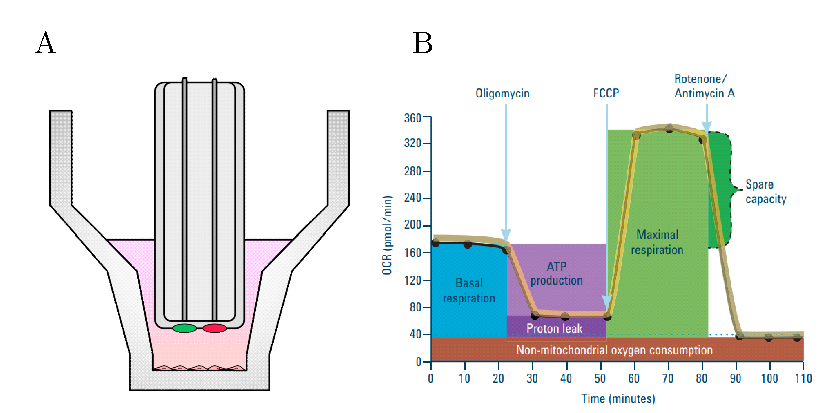
\includegraphics{Abbildung/seahorse_basics_placeholder.pdf}

    \begin{minipage}{\captionwidth}
        \caption[enrichment]{\uzlemph{Basics of Seahorse Assay (a placeholder)}\\
        \textbf{(A)} Schematic of a well used for Seahorse Assay. For the measurement the piston in the middle lowers to the bottom, this way defining a restricted space at the bottom. \ac{ocr} and \ac{eacr} in this volume are measured via two porbes (red and green). \textbf{(B)} Examplary curve for \ac{ocr} recorded over time and extractable properties of the respiratory chain.}
        \label{fig:seahorse_basics}
    \end{minipage}
\end{figure}


    \subsection{Seahorse Assay}
    On the day before the assay the Seahorse XF Analyzer was turned on to calibrate and the XF24 Extracellular Flux Assay Kit catridge was left to equilibrate in Seahorse XF calibrant over night at 37 °C (in non-CO2 environment).\\
    On the day of the assay, cells were washed with 500 µL PBS each and afterwards 500 µL XF BASE medium, supplemented with 1 mM Pyrucate, 10 mM Glucose, 2 mM Glutamine \& 90 µM NaOH, was added. The cells were left to incubate for 1 h at 37°C in non-CO2 environment. During this time toxins for disruption of the respiratory chain were prepared and loaded into the XF24 Extracellular Flux Assay catridge:

    \begin{table}[h]
    \capstart
    \centering
    \begin{minipage}{\captionwidth}
        \caption[toxins for seahorse]{\uzlemph{Toxin Concentrations for XF24 Extracellular Flux Assay}}
        \label{tab:seahorse_toxins}
    \end{minipage}
    \begin{tabular}{|c|c|c|c|}
        \hline
        component  & concentration in cartridge(µM) & volume in cartridge(µL) & concentration in well (µM) \\ \hline
        Oligomycin & 14                             & 55                      & 1.4                        \\
        FCCP       & 10                             & 60                      & 2.0                        \\
        Antimycin  & 50                             & 65                      & 5.0                        \\ \hline
    \end{tabular}
    \end{table}

    The catridge was loaded into the XF Analyser for calibration, after successful calibration the hydration catridge was replaced with the cell plate. Measurement was programmed out as following:

    \begin{itemize}
        \item Calibration of the probes.
        \item Equilibration
        \item 3 Repeats of:
        \begin{itemize}
            \item Mixing (1 min)
            \item Pause (2 min)
            \item Detection of OCR and \ac{ecar} (4 min)
        \end{itemize}
        \item Pause (2 min)
        \item Injection of 55 µL Oligomycin
        \item 3 Repeats of:
        \begin{itemize}
            \item Mixing (1 min)
            \item Pause (2 min)
            \item Detection of OCR and \ac{ecar} (4 min)
        \end{itemize}
        \item Pause (2 min)
        \item Injection of 60 µL FCCP
        \begin{itemize}
            \item Mixing (1 min)
            \item Pause (2 min)
            \item Detection of OCR and \ac{ecar} (4 min)
        \end{itemize}
        \item Pause (2 min)
        \item Injection of 55 µL Antimycin
        \item 3 Repeats of:
        \begin{itemize}
            \item Mixing (1 min)
            \item Pause (2 min)
            \item Detection of OCR and \ac{ecar} (4 min)
        \end{itemize}
    \end{itemize}

    Finally the medium was removed and cells were stained for 15 min with 1 µg/mL Hoechst in \ac{pbs} and photographed to determine cell count for normalization.

    \subsection{Processing of Data}
    Cells were quantified using a python script provided by my supervisor Dr. Tobias Reinberger. \ac{ocr} and \ac{ecar} calculated by the XF Analyzer were normalize in using this cell count and the signal of the control wells.
    In total three biological were recorded of which on was excluded because no changes in \ac{ocr} and \ac{ecar} could be detected and cells deacttched from the bottom of the wells during Hoechst staining. For the remaining two replicates the least fitting of the 5 technical repeats for each condition was manually excluded.
    Further initial \ac{ocr} and \ac{ecar} as well as the characteristics of the respiratory chain displayed in figure \ref{fig:seahorse_basics} B were calculated, again using a modified python script provided by Dr. Tobias Reinberger. Assuming a normal distribution, student's t-test was used, a p-value of 0.05 is considered as significant. For detailed information please check the script.

\section{Oxidative Stress Assay}
\label{sec:cellrox}
CellROX Green is a flourescent dye that gets oxidized in a situation of oxidative stress and then binds to DNA, showing bright green flourescence \cite{CellROXGreenReagent}.
CellROX Green assay was used to assess generation of \ac{ros} in \acp{haosmc} differentiated as described in section \ref{subsec:differentiation}. After further differentiation, further stimulation (from here on refered to as 'boost') with \ac{pdgf} was carried put. Additionally, a recovery experiment was performed using \ac{nac}, a potent anioxidant, to quench generation of \ac{ros}.

    \subsection{CellROX Assay}
For the assay cells were washed with \ac{pbs}, then the boost was performed using variable concentrations of \ac{pdgf} in 300 µL \ac{hbss}. For \ac{ros} quenching with \ac{nac}, 0.25 M \ac{nac} solution was added to the wells 2 h prior to the experient and also added to \ac{hbss} during the experiment.

    \begin{table}[h]
    \capstart
    \centering
    \begin{minipage}{\captionwidth}
        \caption[Seahorse Assay]{\uzlemph{Composition for Seahorse Assay Boost}}
        \label{tab:cellrox_table}
    \end{minipage}
    \begin{tabular}{|c|c|c|c|}
        \hline
        component         & concentration & final concentration      & volume (µL) \\ \hline
        HBSS              & -             & -                        & 300         \\
        PDGF              & ?             & variable (0 - 400 ng/mL) & variable    \\
        Hoechst           & 1 mg/mL       & 1 µg/mL                  & 0.3         \\
        CellROX   (1:500) & 2.5 mM        & 5 µM                     & 0.6         \\
        NAC               & 0.25 M        & variable (0 - 8 mM)      & variable    \\ \hline
        total             & -             & -                        & $\sim$300   \\ \hline
    \end{tabular}
    \end{table}

    Cells were kept at 37°C in 5 \% CO2 environment during the boost, the incubation time is indicated with the results of the respective experiment. Imaging was done with the BZ-X810 All-in-One Flourescence Microscope, using standard sensitivity. Images for the \ac{nac} quench were recorded as a z-stack and merged into one image using [KEYENCE SOFTWARE].

    \subsection{Processing of Data}
    For time resolved \ac{pdgf} boost titration, 7 biological repeats were performed of which one was excluded because of extremly high signal in the negative control. For \ac{nac} quench, 4 biological repeats were performed of which one was excluded because no signal in the positive control.
    For quantification of signal itensity, pixels with a green value higher than 90 were counted. Differences in cell count were adjusted by divison through the number of pixels with a blue value bigger than 80. To adjust for large variance in total signal intensity between biological repeats, values were adjusted by divison through the total signal of all recorded conditions.
    Mann Whitney U Test was used, a p-value of 0.05 is considered as significant. For detailed information please check the scripts.


\section{Curation of Data for postGWAS Analyses}
\label{sec:database}
Dta for postGWAS analyses and co-visualization with the \ac{gwas} data, was downloaded from public resources. Processing of the data and further annotation is briefly described in the follwing listing. The finallay generated tables are summarized in figure \ref{fig:db_er} and table \ref{tab:db_summary}. For a complete view please consult the the download scripts.

\begin{itemize}
    \item \uzlemph{GWAS Summary Statistics:} The \ac{cad} \ac{gwas} summary statistics as well as a list of indetified proxy \acp{snp} from the study were annotated via the ensembl \ac{rest} \ac{api} by Dr. Tobias Reinberger.

    \item \uzlemph{HGNC Gene List} The newest quarterly update to the complete \ac{hgnc} dataset was downloaded via the \MYhref{http://ftp.ebi.ac.uk/pub/databases/genenames/hgnc/archive/}{\ac{hgnc} \ac{ftp} server}. The dataset was used to generate a list of all 43135 approved symbols, mapping to their \ac{hgnc} id as well as a list of all 98723 symbols (approved, alias and previous), mapping to their \ac{hgnc} id.

    \item \uzlemph{Linked SNPs} \ac{ld} $r^2$ values for variants in a 500 kb window around all variants in the list of \ac{cad} \ac{gwas} proxy variants, were computed and downloaded via the \MYhref{https://rest.ensembl.org/documentation/info/ld_id_get}{ensembl \ac{rest} \ac{api}}. For humans ensembl calculates the \ac{ld} with data from the 1000 Genomes project (see table \ref{tab:populations}). In the same process linked \acp{snp} were annotated with their most severe consequence by the ensembl \ac{vep}. In total information for 449770 relationships was downloaded.

    \begin{table}[h]
    \capstart
    \centering
    \begin{minipage}{\captionwidth}
        \caption[1000 Genomes Populations]{\uzlemph{1000 Genomes Populations}}
        \label{tab:populations}
    \end{minipage}
    \begin{tabular}{|c|c|c|}
        \hline
        Name                   & Size (individuals)   & Description      \\ \hline
        1000GENOMES:phase3:ALL & 2504                 & All phase 3 individuals  \\
        1000GENOMES:phase3:AMR & 347                  & Americans  \\
        1000GENOMES:phase3:EAS & 504                  & East Asians  \\
        1000GENOMES:phase3:EUR & 503                  & European \\
        1000GENOMES:phase3:SAS & 489                  & South Asian  \\ \hline
    \end{tabular}
    \end{table}

    \item \uzlemph{Ensembl Genome Annotatation} The newest ensembl build (ensembl release 106) was downloaded via the \MYhref{http://ftp.ensembl.org/pub/current_gtf/homo_sapiens/}{ensembl \ac{ftp} server}. Features annotated as genes of the type protein coding (19994), lncRNA (17734) or miRNA (1877) were extracted, further gene symbols were mapped to their \ac{hgnc} id if possible.

    \item \uzlemph{Ensembl Regulatory Build} The newest ensembl regulatory build (ensembl release 106) was downloaded via the \MYhref{http://ftp.ensembl.org/pub/current_regulation/homo_sapiens/}{ensembl \ac{ftp} server}, containing 110623 open chromatin regions, 30873 \ac{tf} binding sites, 175885 \ac{ctcf} bindsing sites, 127935 enhancers, 36597 promotors \& 140548 promotor flanking regions.

    \item \uzlemph{Open Target Genetics l2g Scores} The lattest list of Open Target Genetics \ac{l2g} Scores was downloaded via the \MYhref{http://ftp.ebi.ac.uk/pub/databases/opentargets/genetics/latest/l2g/}{open target geneitcs \ac{ftp} server}. Entries were annotated with their \ac{hgnc} ID when ever possible, 655 entries that do not map to a gene that is approved by the \ac{hgnc} were dropped, yielding a total of 3580206 database entries.

    \item \uzlemph{TSS} 35160 \ac{tss} for protein coding genes were extracted from a \MYhref{https://ccg.epfl.ch/mga/hg38/gencode/}{\ac{USCS} Genome Brower dump} -> I know this needs improvment, but this is literally the last point on my agenda.

    \item \uzlemph{Associated traits from GWAS catalog} The \ac{snp} trait associations from the lattest release of the GWAS catalog as well as the accompanying list of studies was downloaded via the \MYhref{http://ftp.ebi.ac.uk/'}{GWAS catalog FTP server}. 14892 \ac{snp}-trait correlations missing a the position or a p-value for the association were dropped from the data set. Further the column for Odds Ration or beta was seperated in to two columns. In total 370002 assocciations from 5831 distinct studies were collected.

    \item \uzlemph{TADs} \acp{tad} predicted by software adapted from \textcite{dixonTopologicalDomainsMammalian2012} were downloaded via the 3D genome browser. In total \acp{tad} in 40 distinct biosamples were downloaded.

    \item \uzlemph{scATAC-seq from \textcite{newmanMultipleCellTypes2021a}} Processed sc\ac{atac} data for 8 celltypes [SOME MORE INFO] were scraped from the \MYhref{https://github.com/MillerLab-CPHG/Coronary_snATAC/tree/main/3_SVMpipeline/celltype_peaks}{Miller Lab GitHub repository}.

    \item \uzlemph{scATAC-seq from CATlas} Processed sc\ac{atac} data was scraped from the \MYhref{http://renlab.sdsc.edu/kai/Key_Processed_Data/Peaks/}{Ren Labs website} for 222 biosamples.

    \item \uzlemph{ABC model} The \ac{abc} model data for 131 biosamples was downloaded from the \MYhref{http://ftp.broadinstitute.org/outgoing/lincRNA/ABC/}{Engreitz Lab \ac{ftp} server}. The data was further translated from Hg19 to Hg38 using pyliftover.

    \item \uzlemph{ENCODE cCREs} \acp{cCRE} in  distinct biosamples were downloaded by Dr. Tobias Reinberger, filtering out elements that were annotated \textit{unclassified}.
\end{itemize}

\section{Visualization of GWAS data}
\label{sec:gwas_vis}
For visualization of the data, an bokeh application was build, that fetches the data from the database and renders it to a webbrowser.\\
Bokeh is a python module that allow easy and interactive visualization of data. It combines the powerful data processing tools of python with the interactivity of JavaScript running in the browser. The python side of bokeh creates python objects which are serialized into JSON data and handed over to bokehJS which deserializes them into JavaScript objects that are rendered to the browser. The intergrated bokeh server additionally offers the possiblity to synchronize data between the underlying python environment and brower side JavaScript library, allowing real time updates to the displayed data.

    \begin{figure}[h]
    \capstart
        \centering
    	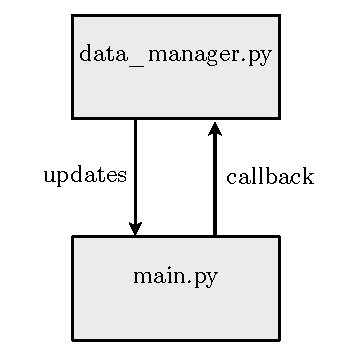
\includegraphics{Abbildung/vis_architecture.pdf}

    	\begin{minipage}{\captionwidth}
    		\caption[vis archi]{\uzlemph{Architecture of the vis tool} \newline }
    		\label{fig:plot_architecture}
    	\end{minipage}
    \end{figure}

According to good design principles the concerns of the application are split into two sections shown in fig. \ref{fig:plot_architecture}. Reading of data from the database and further processing steps are managed by a data provide and enclosed in one class. In contrast to the model-controler-view architecture, a popular architectural pattern for the design of user interfaces, there is no partition between a view and a controler. Since data visualization as well as the control widgets are created by bokeh, it is convienient to use the build in event listeners of the library to handle the required callbacks. Therefore the main file is responsilbe for the creation of all plots and widgets as well as listening for inputs.

\section{Enrichment analysis}
\label{sec:enrichment}
Based on the data in the database an initial postGWAS studies was run. Annotation enrichment analyses are a popular tool for the identification of terms that are over-represent in a list of interest. The most prominent application probably being their application as \ac{gsea}. \acp{gesa} are used to check for the over-representtion of a candidate gene list in a predefined set of genes \cite{tipneyIntroductionEffectiveUse2010}. In this case the method is used to determine if \acp{cCRE} overlap with \ac{cad} associted \acp{snp} is enriched in a biosample, using fisher's exact test.
For the analysis \acp{cCRE} annotated as unclassified were excluded. As a list of \ac{cad} associted \acp{snp} the list of 241 proxy variants from the database was used, as well all linked varinats (r2 >= 0.6) in the 1000 Genomes European Population. The the following parameters were calculated for all biosamples:

\begin{itemize}
    \item The number of distinct cCREs among all biosamples (m)
    \item The number of distinct cCREs that are annotated in the biosample of interest (mt)
    \item The Number of distinct cCREs that overlap with a SNP in the SNP list in any biosample (n)
    \item The Number of distinct cCREs that overlap with a SNP in the SNP list in the biosample of interest (nt)
\end{itemize}

The p-value for the number of overlaps to be greater than or equal to the observation can be calculated as the cumulative distribution function of the hypergeometric distribution.

$$ P(\sigma_t\geq n_t) = \sum_{k=n_t}^{min(m_t, n)} \frac{\binom{n}{k}\binom{m-n}{m_t-k}}{\binom{m}{m_t}} $$

To account for the multiple comparisons problem, p-values were adjusted with Bonferroni correction where n is the number of tests ($\equiv$ number of biosamples):

$$ p_{ajd.} = p*n$$

The analysis and visualization were done in python. A p-value of 0.05 is considered as significant. For detailed information please check the analysis script and the visualization script.

\begin{figure}[h]
\capstart
    \centering
    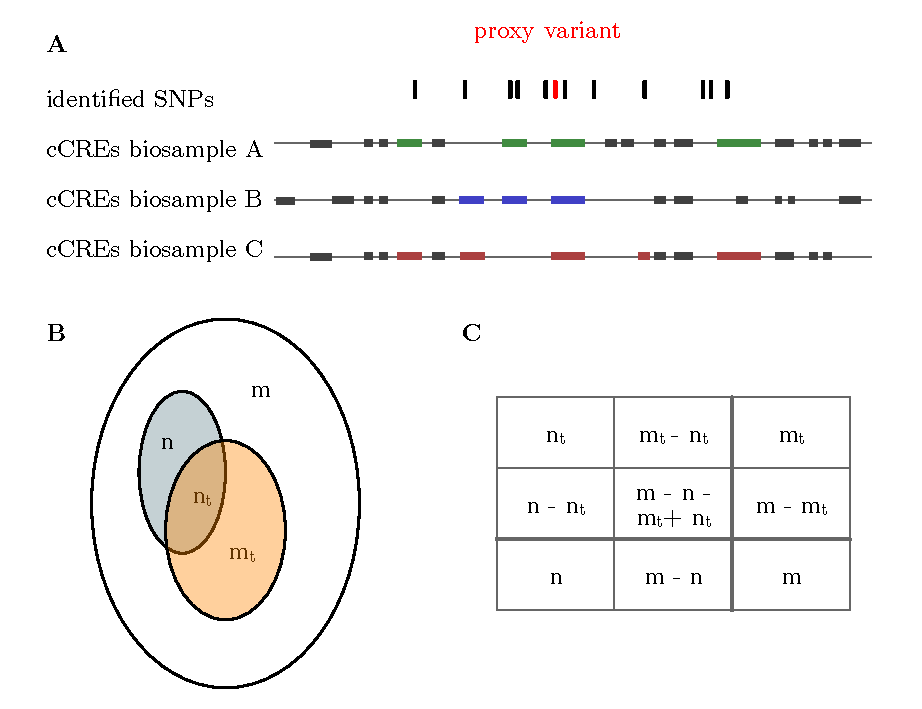
\includegraphics{Abbildung/enrichment.pdf}

    \begin{minipage}{\captionwidth}
        \caption[enrichment]{\uzlemph{Enrichment analysis for \acp{cCREs} overlapping with \ac{cad} risk \acp{snp}}\\
        \textbf{(A)} Visual representation of the overlap calculation for enrichment calculation. The proxy variant is indicated as a red line, variants in \ac{ld} are indicated as black lines. \ac{cCRE} are shown as boxes, those that are overlapping with a \ac{snp} were colored according to the biosample they were annotated in. \textbf{(B)} Venn diagram of these values for a biosample. \textbf{(C)} Schematic contingency table for a biosample. \\
        (m) is the number of distinct \acp{cCRE} found among all biosamples (23 in this example); (mt) the number of distinct \acp{cCRE} annotated in the biosample of interest (16 for biosample A, 14 for biosample b, 14 for biosample C); (n) the number of distinct \acp{cCRE} overlapping with a \ac{snp} (6 in this example);  the number of distinct \acp{cCRE} overlapping with a \ac{snp} in the biosample of interest (4 for biosample A (green), 3 for biosample B (blue), 5 for biosample C (red))}
        \label{fig:enrichment}
    \end{minipage}
\end{figure}
